\section{Método Simplex}
\subsection{Descrição Geral}

\begin{frame}
	\frametitle{Histórico}
	\centering
	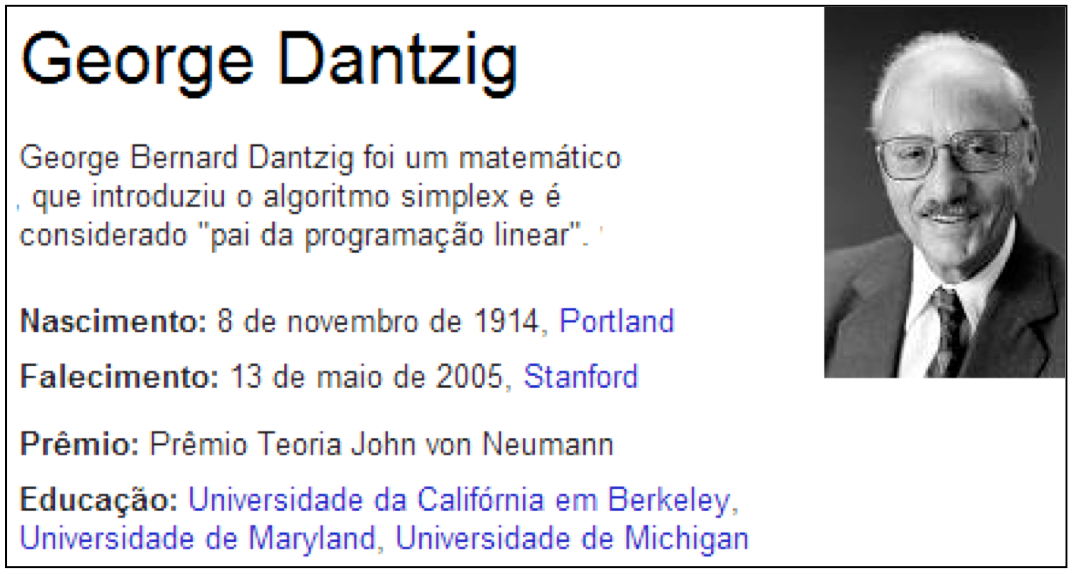
\includegraphics[width=8.5cm,height=5cm]{Dantzig.png}
\end{frame}

\begin{frame}
	\only<1>
	{
	\frametitle{Descrição Geral Simplex}
	}
	\only<2-6>
	{
	\frametitle{Descrição Geral Simplex \scriptsize (SBF = Solução Básica Factível)}
	}
	\centering
	\begin{tikzpicture} [
							auto, node distance = 2cm,
							decisao/.style = { diamond, draw, thick, fill=red!20,
							                   text width=3em, text badly centered,
							                   inner sep=1pt},
							bloco/.style   = { rectangle, draw, thick, fill=blue!20, 
												text width=10em, text centered,
							                   minimum height=1em },
							inicio/.style  = { ellipse, draw, fill=green!20,
							                   text width=5em, text centered },	
							line/.style   = { draw, -latex' },
						]

	    % Place nodes
	    \only<1-6>
	    {
	    \node [inicio] 				                        (init)      {\scriptsize Início: Forma Padrão};
	    }
	    \only<2-6>
	    {
	    \node [bloco,   below of=init]                      (solbasica) {\scriptsize Encontrar uma SBF Inicial};
	    }
	    \only<3-6>
	    {
	    \node [below of=solbasica] 							(null1)		{};
	    \node [decisao, below of=solbasica]                 (decide)    {\scriptsize Solução Ótima ?};
	    }
	    \only<4-6>
	    {
	    \node [bloco,   below of=decide]                    (melhora)   {\scriptsize Determinar uma SBF adjacente melhor};
	    }
	    \only<6>
	    {
	    \node [inicio,  right of=decide, node distance=4cm] (fim)       {\scriptsize Fim};
	    }
	    % Draw edges
	    \only<2-6>
	    {
	    \path [line] (init)      -- (solbasica);
	    }
	    \only<3-6>
	    {
	    \path [line] (solbasica) -- (decide);
	    }
	    \only<4-6>
	    {
	    \path [line] (decide)    -- node [near start] {\scriptsize não} (melhora);
	    }
	    \only<5-6>
	    {
	    \path [line] (melhora)    -| (-3,-2.5)  -- (0,-2.5) (null1);
		}
		\only<6>
		{
	    \path [line] (decide)    -- node [near start] {\scriptsize sim} (fim);
	    } 
	\end{tikzpicture}
\end{frame}

\subsection{Forma Padrão}
\begin{frame}
	\frametitle{Forma Padrão}
	\begin{table}
		\begin{tabular}{c c c}
			\only<1-6>
			{
				{\color{red} \textbf{Forma Geral/Original}} 
			} & &
			\only<2-6>
			{ 
				{\color{red} \textbf{Forma Padrão}} 
			} \\
			\only<1-6>
			{
				\cellcolor{blue!20}
				$
					\begin{matrix}
						\max Z = c^Tx \\
						\text{s.a.} \\
						Ax \{  =, \le, \ge \} b  \\
						x \ge 0  \\
					\end{matrix}
				$ 
			} &
			\only<2-6>
			{ 
				
\includegraphics[width=1.5cm,height=0.5cm]{seta.png}
			} &
			\only<2-6>
			{
				\cellcolor{blue!20}
				$
					\begin{matrix}
						\max Z = c^Tx \\
						\text{s.a.} \\
						Ax = b  \\
						x \ge 0  \\
					\end{matrix}
				$ 
			} \\
		\end{tabular}
	\end{table}
	
	\begin{table}
		\centering
		\begin{tabular}{c}
			\only<3-6>
			{
					
\includegraphics[width=0.3cm,height=0.3cm]{tick.png} \hspace{0.1cm}
					\scriptsize Os termos independentes das restrições devem ser não negativos $(b \ge 0)$. \\
			}
			\only<4-6>
			{

					
\includegraphics[width=0.3cm,height=0.3cm]{tick.png} \hspace{0.1cm}
					\scriptsize Todas as restrições na forma de \underline{igualdade} (exceção: não-negatividade). \\
			}
			\only<5-6>
			{
					
\includegraphics[width=0.3cm,height=0.3cm]{tick.png} \hspace{0.1cm}
					\scriptsize \underline{Não-negatividade}: As variáveis de decisão $x$ devem ser não negativas. \\
			}
			\only<6>
			{
					
\includegraphics[width=2.7cm,height=2.7cm]{importante.jpg} \\
					\cellcolor{green!50} \color{red} Sempre é possível escrever um PPL na forma padrão! \\
			}
			
		\end{tabular}
	\end{table}
\end{frame}

\begin{frame}
	\frametitle{Formulação Padrão} 
	\begin{mdframed}[backgroundcolor=blue!20] 
		\only<1>
		{
			\begin{equation*}
				\max z = c_1x_1 + c_2x_2 + \cdots + c_nx_n 
			\end{equation*}
			{\color{red}Sujeito a (restrições de igualdade)} 
			\begin{equation*}
				\begin{matrix}
					a_{11}x_1 + a_{12}x_2 + \cdots + c_{1n}x_n = b_1 \\
					a_{21}x_1 + a_{22}x_2 + \cdots + c_{2n}x_n = b_2 \\
					\vdots \\
					a_{m1}x_1 + a_{m2}x_2 + \cdots + c_{mn}x_n = b_n \\
					x_1, x_2, \cdots, x_n \ge 0 \\
				\end{matrix}
			\end{equation*}
			$n$ variáveis de decisão e $m$ restrições de igualdade.
		}
		\only<2>
		{
			\begin{equation*}
				\max z = \sum_{j=1}^{n}c_jx_j
			\end{equation*}
			{\color{red}Sujeito a (restrições de igualdade)} 
			\begin{equation*}
				\begin{matrix}
					\sum_{j=1}^{n}a_{ij} = b_i & \forall i = 1, 2, \cdots, m \\
					x_j \ge 0 & \forall j = 1, 2, \cdots, n \\
				\end{matrix}
			\end{equation*}
			$n$ variáveis de decisão e $m$ restrições de igualdade.
		}
		\only<3>
		{
			\begin{equation*} 
				\max z = \begin{bmatrix}
							c_1 & c_2 & \cdots & c_n \\
						 \end{bmatrix}
						 \begin{bmatrix}
							 x_1 \\
							 x_2 \\
							 \vdots \\
							 x_n \\
						 \end{bmatrix}
			\end{equation*}
			{\color{red}Sujeito a (restrições de igualdade)} 
			\begin{equation*}
				\begin{bmatrix}
						a_{11} & a_{12} & \cdots & a_{1n} \\
						a_{21} & a_{22} & \cdots & a_{2n} \\
						\vdots & \vdots & \ddots & \vdots \\
						a_{m1} & a_{m2} & \cdots & a_{mn} \\
				\end{bmatrix}
				\begin{bmatrix}
						x_1 \\
						x_2 \\
						\vdots \\
						x_n \\
				\end{bmatrix} = 
				\begin{bmatrix}
						b_1 \\
						b_2 \\
						\vdots \\
						b_m \\
				\end{bmatrix} \text{ e }
				\begin{bmatrix}
						x_1 \\
						x_2 \\
						\vdots \\
						x_n \\
				\end{bmatrix} \ge
				\begin{bmatrix}
						0 \\
						0 \\
						\vdots \\
						0 \\
				\end{bmatrix} 				
			\end{equation*}			
			$n$ variáveis de decisão e $m$ restrições de igualdade.
		}
		\only<4>
		{
			\begin{equation*} 
				\max z = \begin{bmatrix}
							c_1 & c_2 & \cdots & c_n \\
						 \end{bmatrix}_{\text{\color{red}1 x n}}
						 \begin{bmatrix}
							 x_1 \\
							 x_2 \\
							 \vdots \\
							 x_n \\
						 \end{bmatrix}_{\text{\color{red}n x 1}} 
			\end{equation*}
			{\color{red}Sujeito a (restrições de igualdade)} 
			\begin{equation*}
				\begin{bmatrix}
						a_{11} & a_{12} & \cdots & a_{1n} \\
						a_{21} & a_{22} & \cdots & a_{2n} \\
						\vdots & \vdots & \ddots & \vdots \\
						a_{m1} & a_{m2} & \cdots & a_{mn} \\
				\end{bmatrix}_{\text{\color{red}m x n}}
				\begin{bmatrix}
						x_1 \\
						x_2 \\
						\vdots \\
						x_n \\
				\end{bmatrix}_{\text{\color{red} n x 1}} = 
				\begin{bmatrix}
						b_1 \\
						b_2 \\
						\vdots \\
						b_m \\
				\end{bmatrix}_{\text{\color{red} m x 1}}  				
			\end{equation*}			
			$n$ variáveis de decisão e $m$ restrições de igualdade.
		}
		\only<5>
		{
			\begin{equation*} 
				\max z = \mathbf{c}^T \mathbf{x}
			\end{equation*}
			{\color{red}Sujeito a (restrições de igualdade)} 
			\begin{equation*}
				\begin{matrix}
					\mathbf{A_{eq}x} = \mathbf{B_{eq}}  \\
					\mathbf{x} \ge \mathbf{0}
				\end{matrix}
			\end{equation*}	
			$n$ variáveis de decisão e $m$ restrições de igualdade.		
		}		
	\end{mdframed}
	\only<5>
	{
	\vspace{0.3cm}
	\begin{equation*}
		\begin{matrix}
			\mathbf{c} = 	\begin{bmatrix}
									c_1 \\ c_2 \\ \vdots \\ c_n \\
							\end{bmatrix} &

			\mathbf{x} = 	\begin{bmatrix}
									x_1 \\ x_2 \\ \vdots \\ x_n \\
							\end{bmatrix} &

			\mathbf{B_{eq}} = 	\begin{bmatrix}
									b_1 \\ b_2 \\ \vdots \\ b_m \\
							\end{bmatrix} &

			\mathbf{A_{eq}} = 	\begin{bmatrix}
									a_{11} & a_{12} & \cdots & a_{1n} \\
									a_{21} & a_{22} & \cdots & a_{2n} \\
									\vdots & \vdots & \ddots & \vdots \\
									a_{m1} & a_{m2} & \cdots & a_{mn} \\
								\end{bmatrix} \\

		\end{matrix}
	\end{equation*}
	}
\end{frame}

\begin{frame}
	\frametitle{Relação entre Maximização e Minimização}
	\only<1>
	{
		\centering
		
\includegraphics[width=5cm,height=4cm]{up-down.jpg}
	}	
	\only<2>
	{
		\centering
		
\includegraphics[width=5cm,height=4cm]{up-down.jpg}
		\begin{itemize}
		\item Qualquer que seja o formato do PPL, sempre é possível transforma-lo no formato padrão apresentado.
		\item Como é a relação entre minimização e maximização?
		\end{itemize}
	}	
	\only<3>
	{
		\centering
		
\includegraphics[width=2.5cm,height=2cm]{up-down.jpg}
		\begin{mdframed}[backgroundcolor=blue!20] 
			\begin{equation*}
				\max z = \sum_{j=1}^{n}c_jx_j \Leftrightarrow \min (-z) = \sum_{j=1}^{n}(-c_j)x_j
			\end{equation*}
			\begin{equation*}
				\min z = \sum_{j=1}^{n}c_jx_j \Leftrightarrow \max (-z) = \sum_{j=1}^{n}(-c_j)x_j
			\end{equation*}
		\end{mdframed}
	}
\end{frame}

\begin{frame}
	\frametitle{Relação Entre Inequações e Equações}
	
	\only<1->
	{
	\underline{Restrições de Menor ou Igual} - Variável de Folga ($+S_i$)
	\begin{mdframed}[backgroundcolor=blue!20]
		\begin{equation*}
			\sum_{j-1}^{n}a_{ij}x_j \le b_i \Leftrightarrow
			\left\{ \begin{matrix}
						\sum_{j=1}^{n}a_{ij}x_j + S_i = b_i \\
						0 \le S_i \ge \infty
					\end{matrix}  
			\right.
		\end{equation*}
	\end{mdframed}	
	}
	
	\only<2>
	{
	\vspace{0.5cm}
	\underline{Restrições de Maior ou Igual} - Variável de Excesso ($-S_i$)
	\begin{mdframed}[backgroundcolor=red!20]
		\begin{equation*}
			\sum_{j-1}^{n}a_{ij}x_j \ge b_i \Leftrightarrow
			\left\{ \begin{matrix}
						\sum_{j=1}^{n}a_{ij}x_j - S_i = b_i \\
						0 \le S_i \ge \infty
					\end{matrix}  
			\right.
		\end{equation*}
	\end{mdframed}
	}
\end{frame}

\begin{frame}
	\frametitle{Tratamento de Limites das Variáveis}
	\only<1->
	{
	\underline{Limite Inferior ou \textit{Lower  Bound}}
	\begin{mdframed}[backgroundcolor=blue!20]
		\begin{equation*}
			x_j \ge LB \Leftrightarrow
			\left\{ \begin{matrix}
						x_j - LB = {x}'_j \Rightarrow x_j = {x}'_j + LB \\
						{x}'_j \ge 0
					\end{matrix}  
			\right.
		\end{equation*}
	\end{mdframed}	
	}
	
	\only<2->
	{
	\vspace{0.5cm}
	\underline{Limite Superior ou \textit{Upper  Bound}}
	\begin{mdframed}[backgroundcolor=red!20]
		\begin{equation*}
			x_j \le UB \Leftrightarrow
			\left\{ \begin{matrix}
						UB - x_j = {x}'_j \Rightarrow x_j = UB - {x}'_j  \\
						{x}'_j \ge 0
					\end{matrix}  
			\right.
		\end{equation*}
	\end{mdframed}
	}

	\only<3->
	{
	\vspace{0.5cm}
	\begin{mdframed}[backgroundcolor=green!20]
		\begin{equation*}
			- \infty \le x_j \le \infty \Leftrightarrow
			\left\{ \begin{matrix}
						x_j = {x}'_j - {x}''_j \\
						{x}'_j \ge 0 \text{ e } {x}''_j \ge 0  \\
					\end{matrix}  
			\right.
		\end{equation*}
	\end{mdframed}
	}
\end{frame}

\begin{frame}
	\frametitle{Exemplo 1}
	\begin{columns}
		\only<1-2>
		{
		\begin{column}{0.4\textwidth}
			\centering
			\begin{equation*}
				\overset{\text{\color{red}Forma Original}}
				{
					\overbrace{
								\begin{matrix}
									\max Z = 3x_1 + 2.5x_2 + 1.2x_3 \\
									\text{Sujeito a} \\
									\begin{matrix}
										x_1-2x_2+4x_3 & \le & 40 \\
										x_1+x_2+ 2x_3 & \le & 60 \\
										2x_1+3x_2+x_3 & \ge & 15 \\
									\end{matrix} \\
									x_1, x_2, x_3 \ge 0 \\
								\end{matrix}
							  }
				}
			\end{equation*}
		\end{column}
		}
		\only<2>
		{
		\begin{column}{0.6\textwidth}
			\centering
			\begin{equation*}
				\overset{\text{\color{red}Forma Padrão}}
				{
					\overbrace{
								\begin{matrix}
									\max Z = 3x_1 + 2.5x_2 + 1.2x_3 \\
									\text{Sujeito a} \\
									\begin{matrix}
										x_1-2x_2+4x_3 & \cellcolor{red!20}+x_4 &      &      & = & 40 \\
										x_1+x_2+2x_3  &      & \cellcolor{red!20}+x_5 &      & = & 60 \\
										2x_1+3x_2+x_3 &      &      & \cellcolor{red!20}-x_6 & = & 15 \\
									\end{matrix} \\
									x_1, x_2, x_3, x_4, x_5, x_6 \ge 0 \\
								\end{matrix}
							  }
				}
			\end{equation*}
		\end{column}
		}
	\end{columns}
\end{frame}

\begin{frame}
	\frametitle{Exemplo 2}
	\begin{columns}
		\begin{column}{0.5\textwidth}
		\begin{block}{Coloque o PPL abaixo na \underline{forma padrão}.}
			\begin{equation*}
				\begin{matrix}
					\scriptstyle \max Z = -2x_1+x_2+x_3-3x_4+x_5 \\
					\scriptstyle \text{Sujeito a:} \\
					\scriptstyle x_1+2x_2-x_3+x_4+3x_5 \ge 5 \\
					\scriptstyle 4x_1+x_3-2x_4-x_5 \le 0 \\
					\scriptstyle -2x_3+x_4+2x_5\ge -7 \\
					\scriptstyle 3x_1+x_2-x_4+x_5 = 8 \\
					\scriptstyle x_3 \le 0 \\
					\scriptstyle x_4 \text{ qualquer} \\
					\scriptstyle x_1, x_2, x_5 \ge 0 \\
				\end{matrix}
			\end{equation*}
		\end{block}
		\end{column}
		\begin{column}{0.5\textwidth}
			\begin{exampleblock}{Resposta: PPL Escrito na \underline{Forma Padrão}.}
				\begin{equation*}
					\begin{matrix}
						\only<2-9>{\scriptstyle \max Z = -2x_1+x_2+x_3-3x_4+x_5 \\}
						\only<3-9>{\scriptstyle \text{Sujeito a:} \\}
						\only<3-9>{\scriptstyle x_1+2x_2-x_3+x_4+3x_5 {\color{red}-S_1} = 5 \\}
						\only<4-9>{\scriptstyle 4x_1+x_3-2x_4-x_5 {\color{red}+S_2} = 0 \\}
						\only<5-9>{\scriptstyle {\color{red}2x_3-x_4-2x_5 +S_3 = 7} \\}
						\only<6-9>{\scriptstyle 3x_1+x_2-x_4+x_5 = 8 \\}
						\only<7-9>{\scriptstyle {\color{red}x_3=-x'_3 } \\}
						\only<8-9>{\scriptstyle {\color{red}x_4 = x'_4 - x''_4} \\}
						\only<9-9>{\scriptstyle x_1, x_2, {\color{red}x'_3, x'_4, x''_4, S_1, S_2, S_3,} x_5 \ge 0 \\}

						\only<10>{\scriptstyle \max Z = -2x_1+x_2{\color{red}-x'_3}-3{\color{red}(x'_4 - x''_4)}+x_5 \\}
						\only<10>{\scriptstyle \text{Sujeito a:} \\}
						\only<10>{\scriptstyle x_1+2x_2{+x'_3}{\color{red}+x'_4 - x''_4}+3x_5 {\color{red}-S_1} = 5 \\}
						\only<10>{\scriptstyle 4x_1{-x'_3}-2{\color{red}(x'_4 - x''_4)}-x_5 {\color{red}+S_2} = 0 \\}
						\only<10>{\scriptstyle {\color{red}-2{\color{red}x'_3}-{\color{red}(x'_4 - x''_4)}-2x_5 +S_3 = 7} \\}
						\only<10>{\scriptstyle 3x_1+x_2-{\color{red}(x'_4 - x''_4)}+x_5 = 8 \\}
						\only<10>{\scriptstyle x_1, x_2, {\color{red}x'_3, x'_4, x''_4, S_1, S_2, S_3,} x_5 \ge 0 \\}


					\end{matrix}
				\end{equation*}
			\end{exampleblock}
		\end{column}
	\end{columns}
\end{frame}

\begin{frame}[fragile]
	\frametitle{Exemplo 2}
	\begin{columns}
		\begin{column}{0.5\textwidth}
		\begin{block}{Coloque o PPL abaixo na \underline{forma padrão}.}
			\begin{equation*}
				\begin{matrix}
					\scriptstyle \max Z = -2x_1+x_2+x_3-3x_4+x_5 \\
					\scriptstyle \text{Sujeito a:} \\
					\scriptstyle x_1+2x_2-x_3+x_4+3x_5 \ge 5 \\
					\scriptstyle 4x_1+x_3-2x_4-x_5 \le 0 \\
					\scriptstyle -2x_3+x_4+2x_5\ge -7 \\
					\scriptstyle 3x_1+x_2-x_4+x_5 = 8 \\
					\scriptstyle x_3 \le 0 \\
					\scriptstyle x_4 \text{ qualquer} \\
					\scriptstyle x_1, x_2, x_5 \ge 0 \\
				\end{matrix}
			\end{equation*}
		\end{block}
		\end{column}
		\begin{column}{0.5\textwidth}
			\begin{block}{Programa em Matlab}
				\begin{lstlisting}[basicstyle=\tiny]  
clear all; close all; clc;
c = -[-2 1 1 -3 1];
A = [-1 -2 1 -1 -3; ...
      4  0 1 -2 -1; ...
      0  0 2 -1 -2];
B = [-5; 0 ; 7];
Aeq = [3 1 0 -1 1];
Beq = 8;
LB = [0     0 -inf -inf   0]; 
UB = [inf inf    0 inf  inf];
[x,fval, exitflag] = linprog(c,A,B,Aeq,Beq,LB,UB);
				\end{lstlisting}
			\end{block}
		\end{column}
	\end{columns}
\end{frame}

\begin{frame}
	\frametitle{Exemplo 2}
	\begin{columns}
		\begin{column}{0.5\textwidth}
		\begin{block}{Coloque o PPL abaixo na \underline{forma padrão}.}
			\begin{equation*}
				\begin{matrix}
					\scriptstyle \max Z = -2x_1+x_2+x_3-3x_4+x_5 \\
					\scriptstyle \text{Sujeito a:} \\
					\scriptstyle x_1+2x_2-x_3+x_4+3x_5 \ge 5 \\
					\scriptstyle 4x_1+x_3-2x_4-x_5 \le 0 \\
					\scriptstyle -2x_3+x_4+2x_5\ge -7 \\
					\scriptstyle 3x_1+x_2-x_4+x_5 = 8 \\
					\scriptstyle x_3 \le 0 \\
					\scriptstyle x_4 \text{ qualquer} \\
					\scriptstyle x_1, x_2, x_5 \ge 0 \\
				\end{matrix}
			\end{equation*}
		\end{block}
		\end{column}
		\begin{column}{0.5\textwidth}
			\begin{block}{Programa em Matlab}
				\only<1>
				{
					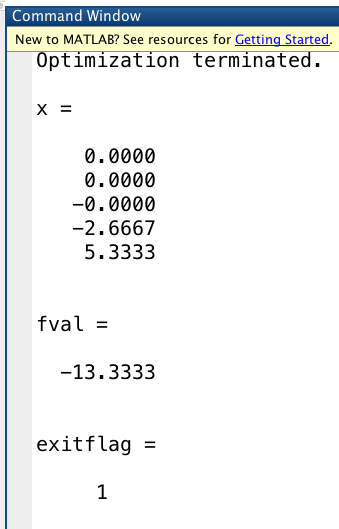
\includegraphics[width=4cm,height=6.5cm]{Exemplo2a.png}
				}
				\only<2>
				{
					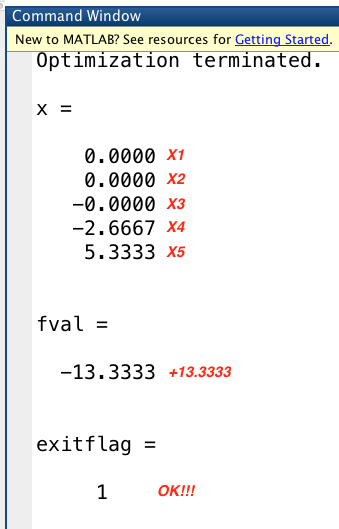
\includegraphics[width=4cm,height=6.5cm]{Exemplo2aLINHA.png}
				}
			\end{block}
		\end{column}
	\end{columns}
\end{frame}

\begin{frame}[fragile]
	\frametitle{Exemplo 2}
	\begin{columns}
		\begin{column}{0.5\textwidth}
			\begin{exampleblock}{Resposta: PPL Escrito na \underline{Forma Padrão}.}
				\begin{equation*}
					\begin{matrix}
						\scriptstyle \max Z = -2x_1+x_2{\color{red}-x'_3}-3{\color{red}(x'_4 - x''_4)}+x_5 \\
						\scriptstyle \text{Sujeito a:} \\
						\scriptstyle x_1+2x_2{+x'_3}{\color{red}+x'_4 - x''_4}+3x_5 {\color{red}-S_1} = 5 \\
						\scriptstyle 4x_1{-x'_3}-2{\color{red}(x'_4 - x''_4)}-x_5 {\color{red}+S_2} = 0 \\
						\scriptstyle {\color{red}-2{\color{red}x'_3}-{\color{red}(x'_4 - x''_4)}-2x_5 +S_3 = 7} \\
						\scriptstyle 3x_1+x_2-{\color{red}(x'_4 - x''_4)}+x_5 = 8 \\
						\scriptstyle x_1, x_2, {\color{red}x'_3, x'_4, x''_4, S_1, S_2, S_3,} x_5 \ge 0 \\
					\end{matrix}
				\end{equation*}
			\end{exampleblock}
		\end{column}
		\begin{column}{0.5\textwidth}
			\begin{block}{Programa em Matlab}
				\begin{lstlisting}[basicstyle=\tiny]  
clear all; close all; clc;
c = -[-2 1 -1 -3 +3 1 0 0 0];
A = [];
B = [];
Aeq = [ ...
  1 2  1  1 -1  3 -1 0 0; ...
  4 0 -1  2  2 -1  0 1 0; ...
  0 0 -2 -1  1 -2  0 0 1; ...
  3 1  0 -1  1  1  0 0 0; ...
  ];
Beq = [ 5; 0; 7; 8];
LB = [ 0 0 0 0 0 0 0 0]; 
UB = [inf inf inf inf inf inf inf];
[x,fval, exitflag] = linprog(c,A,B,Aeq,Beq,LB,UB);				
				\end{lstlisting}
			\end{block}
		\end{column}
	\end{columns}
\end{frame}

\begin{frame}
	\frametitle{Exemplo 2}
	\begin{columns}
		\begin{column}{0.5\textwidth}
			\begin{exampleblock}{Resposta: PPL Escrito na \underline{Forma Padrão}.}
				\begin{equation*}
					\begin{matrix}
						\scriptstyle \max Z = -2x_1+x_2{\color{red}-x'_3}-3{\color{red}(x'_4 - x''_4)}+x_5 \\
						\scriptstyle \text{Sujeito a:} \\
						\scriptstyle x_1+2x_2{+x'_3}{\color{red}+x'_4 - x''_4}+3x_5 {\color{red}-S_1} = 5 \\
						\scriptstyle 4x_1{-x'_3}-2{\color{red}(x'_4 - x''_4)}-x_5 {\color{red}+S_2} = 0 \\
						\scriptstyle {\color{red}-2{\color{red}x'_3}-{\color{red}(x'_4 - x''_4)}-2x_5 +S_3 = 7} \\
						\scriptstyle 3x_1+x_2-{\color{red}(x'_4 - x''_4)}+x_5 = 8 \\
						\scriptstyle x_1, x_2, {\color{red}x'_3, x'_4, x''_4, S_1, S_2, S_3,} x_5 \ge 0 \\
					\end{matrix}
				\end{equation*}
			\end{exampleblock}
		\end{column}
		\begin{column}{0.5\textwidth}
			\begin{block}{Programa em Matlab}
				\only<1>
				{
				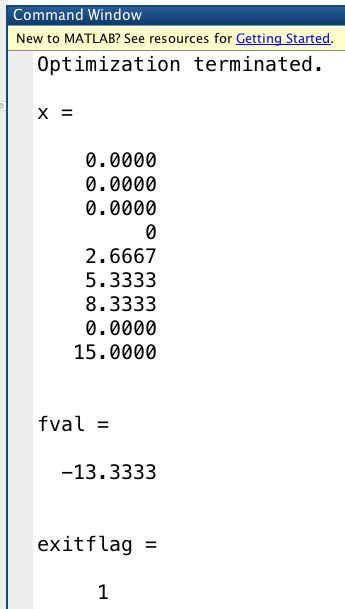
\includegraphics[width=4cm,height=6.5cm]{Exemplo2b.png}
				}
				\only<2>
				{
					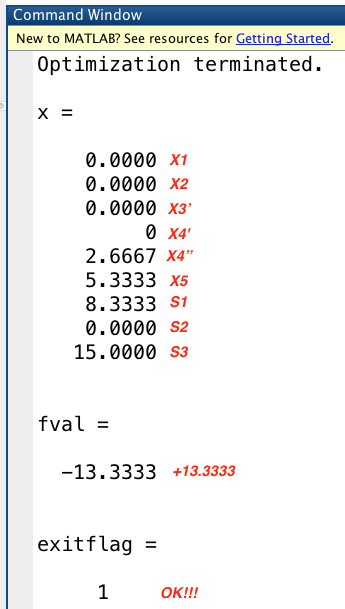
\includegraphics[width=4cm,height=6.5cm]{Exemplo2bLINHA.png}
				}
			\end{block}
		\end{column}
	\end{columns}
\end{frame}

\begin{frame}
	\frametitle{Solução Básica Inicial}
	\begin{block}{\underline{Observações}}
		\begin{enumerate}
			\item A passagem para forma padrão se faz pelo simples acréscimo de uma variável de folga ou excesso para cada inequação existente \pause
			\item {A forma padrão resultante consiste em um sistema que tenha uma \underline{\color{red}solução básica inicial} mais fácil de ser encontrada:} \pause
			\begin{itemize}
				\item[] {\color{red} Solução Básica Inicial (ESTRATÉGIA):} 
					\begin{table}
						\centering		
						\begin{tabular}{c}
							\scriptsize \cellcolor{yellow!70} Anular as variáveis originais \\
							\scriptsize \cellcolor{yellow!70} Obter os valores das variáveis de folga e excesso \\ \pause
						\end{tabular}
					\end{table}
			\end{itemize}
			\item As {\color{red}variáveis nulas} recebem o nome de {\color{red}NÃO BÁSICAS (VNB)} \\
			\item As {\color{red}variáveis não nulas} recebem o nome de {\color{red}BÁSICAS (VB)} \\
		\end{enumerate}
	\end{block}
\end{frame}

\begin{frame}
	\frametitle{Exemplo: Encontre uma {\color{red}\underline{SBF Inicial}} para:}
	\begin{columns}
		\begin{column}{0.3\textwidth}
			\begin{equation*}
				\begin{matrix}
					\scriptstyle \max Z = 3x_1 + 2,5x_2 + 1,2x_3 \\
					\scriptstyle \text{Sujeito a} \\
					\scriptstyle x_1 - 2x_2 + 4x_3 \le 40 \\
					\scriptstyle x_1 + x_2 + 2x_3 \le 60 \\
					\scriptstyle 2x_1 + 3x_2 + x_3 \ge 15 \\
					\scriptstyle x_1, x_2, x_3 \ge 0 \\
				\end{matrix}
			\end{equation*} \pause
		\end{column}
		\begin{column}{0.15\textwidth}
			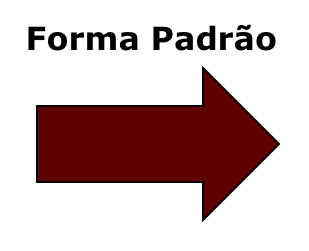
\includegraphics[width=2cm,height=1.5cm]{SetaFormaPadrao.png}
		\end{column}		
		\begin{column}{0.55\textwidth}
			\begin{mdframed}[backgroundcolor=yellow]
				\begin{equation*}
					\begin{matrix}
						\scriptstyle \max Z = 3x_1 + 2,5x_2 + 1,2x_3 \\
						\scriptstyle \text{Sujeito a} \\
					\end{matrix}
				\end{equation*}
				\only<2>
				{
					\begin{equation*}			
					\begin{matrix}
						\scriptstyle x_1 - 2x_2 + 4x_3 & \cellcolor{red!50} \scriptstyle+x_4 & & & \scriptstyle = 40 \\
						\scriptstyle x_1 + x_2 + 2x_3  & & \cellcolor{red!50} \scriptstyle+x_5 & & \scriptstyle = 60 \\
						\scriptstyle 2x_1 + 3x_2 + x_3 & & & \cellcolor{red!50} \scriptstyle-x_6 & \scriptstyle = 15 \\
					\end{matrix}
					\end{equation*}
					\begin{equation*}
					\scriptstyle x_1, x_2, x_3, x_4, x_5, x_6 \ge 0 
					\end{equation*}
				}			
				\only<3>
				{
					\begin{equation*}			
					\begin{matrix}
					\scriptstyle x_1 - 2x_2 + 4x_3 & \cellcolor{red!50} \scriptstyle+x_4 & & & \scriptstyle = 40 \\
					\scriptstyle x_1 + x_2 + 2x_3  & & \cellcolor{red!50} \scriptstyle+x_5 & & \scriptstyle = 60 \\
					\scriptstyle 2x_1 + 3x_2 + x_3 & & & \cellcolor{red!50} \scriptstyle-x_6 & \scriptstyle = 15 \\
					\scriptstyle \cellcolor{red!50} x_6 = -x_6^{*} & & & &\\
					\end{matrix}
					\end{equation*}
					\begin{equation*}
					\scriptstyle x_1, x_2, x_3, x_4, x_5, x_6 \ge 0 
					\end{equation*}
				}			
				\only<4-6>
				{
					\begin{equation*}			
					\begin{matrix}
					\scriptstyle x_1 - 2x_2 + 4x_3 & \cellcolor{red!50} \scriptstyle+x_4 & & & \scriptstyle = 40 \\
					\scriptstyle x_1 + x_2 + 2x_3  & & \cellcolor{red!50} \scriptstyle+x_5 & & \scriptstyle = 60 \\
					\scriptstyle 2x_1 + 3x_2 + x_3 & & & \cellcolor{red!50} \scriptstyle+x_6^{*} & \scriptstyle = 15 \\
					\end{matrix}
					\end{equation*}
					\begin{equation*}
					\scriptstyle x_1, x_2, x_3, x_4, x_5, x_6^{*} \ge 0 
					\end{equation*}
				}			
			\end{mdframed}
		\end{column}
	\end{columns}
	
	\only<5-6>
	{
		\begin{block}{Solução Básica Factível Inicial ???}
			\only<5>
			{
			\begin{itemize}
				\item As {\color{red}variáveis nulas} recebem o nome de {\color{red}NÃO BÁSICAS (VNB)}
				\item As {\color{red}variáveis não nulas} recebem o nome de {\color{red}BÁSICAS (VB)} 
			\end{itemize}
			}
			\only<6>
			{
				\begin{equation*}
					\begin{matrix}
						VNB = \{ x_1,x_2,x_3 \} \Leftrightarrow x_1=0, x_2=0, x_3=0 \\
						VB = \{ x_4,x_5,x_6^{*} \} \Leftrightarrow x_4=40, x_5=60, x_6^{*}=15 \\
						Z = 0 \\
					\end{matrix}
				\end{equation*}
			}
		\end{block}
	}

\end{frame}


\subsection{Passos da Resolução do PPL via Tableau Simplex}

\begin{frame}
	\frametitle{Passos da Resolução do PPL via Tableau Simplex}
	\begin{columns}
		\begin{column}{0.10\textwidth}
			\centering
			\only<2>
			{
				
\includegraphics[width=2.5cm,height=2.5cm]{number_1.jpg}\\
			}
			\only<3>
			{
				
\includegraphics[width=2.5cm,height=2.5cm]{number_2.jpg}\\
			}
			\only<4-5>
			{
				
\includegraphics[width=2.5cm,height=2.5cm]{number_3.jpg}\\
			}
			\only<6>
			{
				
\includegraphics[width=2.5cm,height=2.5cm]{number_4.jpg}\\
			}
		\end{column}
		\begin{column}{0.3\textwidth}
			\centering
			\begin{table}
				\only<1>
				{
				\begin{tabular}{c}
					\cellcolor{yellow}Problema em Análise \\
					$
						\begin{matrix}
							\max Z = 3x_1 + 5x_2 \\
							\text{Sujeito a:} \\
							x_1 \le 4 \\
							2x_2 \le 12 \\
							3x_1 + 2x_2 \le 18 \\
							x_1, x_2 \ge 0 \\
						\end{matrix} 	
					$ \\
				\end{tabular}
				}
				\only<2>
				{
				\begin{tabular}{c}
					\cellcolor{yellow}Problema em Análise \\
					\cellcolor{red!60}\scriptsize Reescrever a expressão da FOB \\ 
					$
						\begin{matrix}
							\color{red} \max Z - 3x_1 - 5x_2 = 0 \\
							\text{Sujeito a:} \\
							x_1 \le 4 \\
							2x_2 \le 12 \\
							3x_1 + 2x_2 \le 18 \\
							x_1, x_2 \ge 0 \\
						\end{matrix} 	
					$ \\
				\end{tabular}
				}		
				\only<3>
				{
				\begin{tabular}{c}
					\cellcolor{yellow}Problema em Análise \\
					\cellcolor{red!60}\scriptsize Problema na Forma Padrão \\ 
					$
						\begin{matrix}
							\color{red} \max Z - 3x_1 - 5x_2 = 0 \\
							\text{Sujeito a:} \\
							x_1 + {\color{red}S_1 =} 4 \\
							2x_2 + {\color{red}S_2 =} 12 \\
							3x_1 + 2x_2 + {\color{red}S_3 =} 18 \\
							x_1, x_2,{\color{red} S_1, S_2, S_3} \ge 0 \\
						\end{matrix} 	
					$ \\
				\end{tabular}
				}		
				\only<4-5>
				{
				\begin{tabular}{c}
					\cellcolor{yellow}Problema em Análise \\
					\cellcolor{red!60}\scriptsize Achar SBF Inicial \\
					$
						\begin{matrix}
							\color{red} \max Z - 3x_1 - 5x_2 = 0 \\
							\text{Sujeito a:} \\
							x_1 + {\color{red}S_1 =} 4 \\
							2x_2 + {\color{red}S_2 =} 12 \\
							3x_1 + 2x_2 + {\color{red}S_3 =} 18 \\
							x_1, x_2,{\color{red} S_1, S_2, S_3} \ge 0 \\
						\end{matrix} 	
					$ \\
					\hline
					$
					\begin{matrix}
						\cellcolor{red!60}S_1 = 4  & \cellcolor{red!60}x_1 = 0 \\
						\cellcolor{red!60}S_2 = 12 & \cellcolor{red!60}x_2 = 0 \\
						\cellcolor{red!60}S_3 = 18 & \cellcolor{red!60}Z = 0 \\
					\end{matrix}
					$ \\
					\hline
				\end{tabular}
				}						
				\only<6>
				{
				\begin{tabular}{c}
					\cellcolor{yellow}Problema em Análise \\
					\cellcolor{red!60}\scriptsize Montar o TABLEAU Simplex \\
					$
						\begin{matrix}
							\color{red} \max Z - 3x_1 - 5x_2 = 0 \\
							\text{Sujeito a:} \\
							x_1 + {\color{red}S_1 =} 4 \\
							2x_2 + {\color{red}S_2 =} 12 \\
							3x_1 + 2x_2 + {\color{red}S_3 =} 18 \\
							x_1, x_2,{\color{red} S_1, S_2, S_3} \ge 0 \\
						\end{matrix} 	
					$ \\
					\hline
					$
					\begin{matrix}
						\cellcolor{red!60}S_1 = 4  & \cellcolor{red!60}x_1 = 0 \\
						\cellcolor{red!60}S_2 = 12 & \cellcolor{red!60}x_2 = 0 \\
						\cellcolor{red!60}S_3 = 18 & \cellcolor{red!60}Z = 0 \\
					\end{matrix}
					$ \\
					\hline
				\end{tabular}
				}						
			\end{table}
		\end{column}
		\centering
		\begin{column}{0.4\textwidth}
			\centering
			\only<5>
			{
				\begin{tabular}{c}
					\hline
					$
						VNB = \{ x_1, x_2 \} 
					$ \\
					$
						VB = \{ S_1, S_2, S_3 \} 
					$ \\
					\hline
				\end{tabular}
				\begin{alertblock}{Atenção}
					A FOB deve ser sempre formada por VNB.
				\end{alertblock}
				
			}		
			\only<6>
			{
				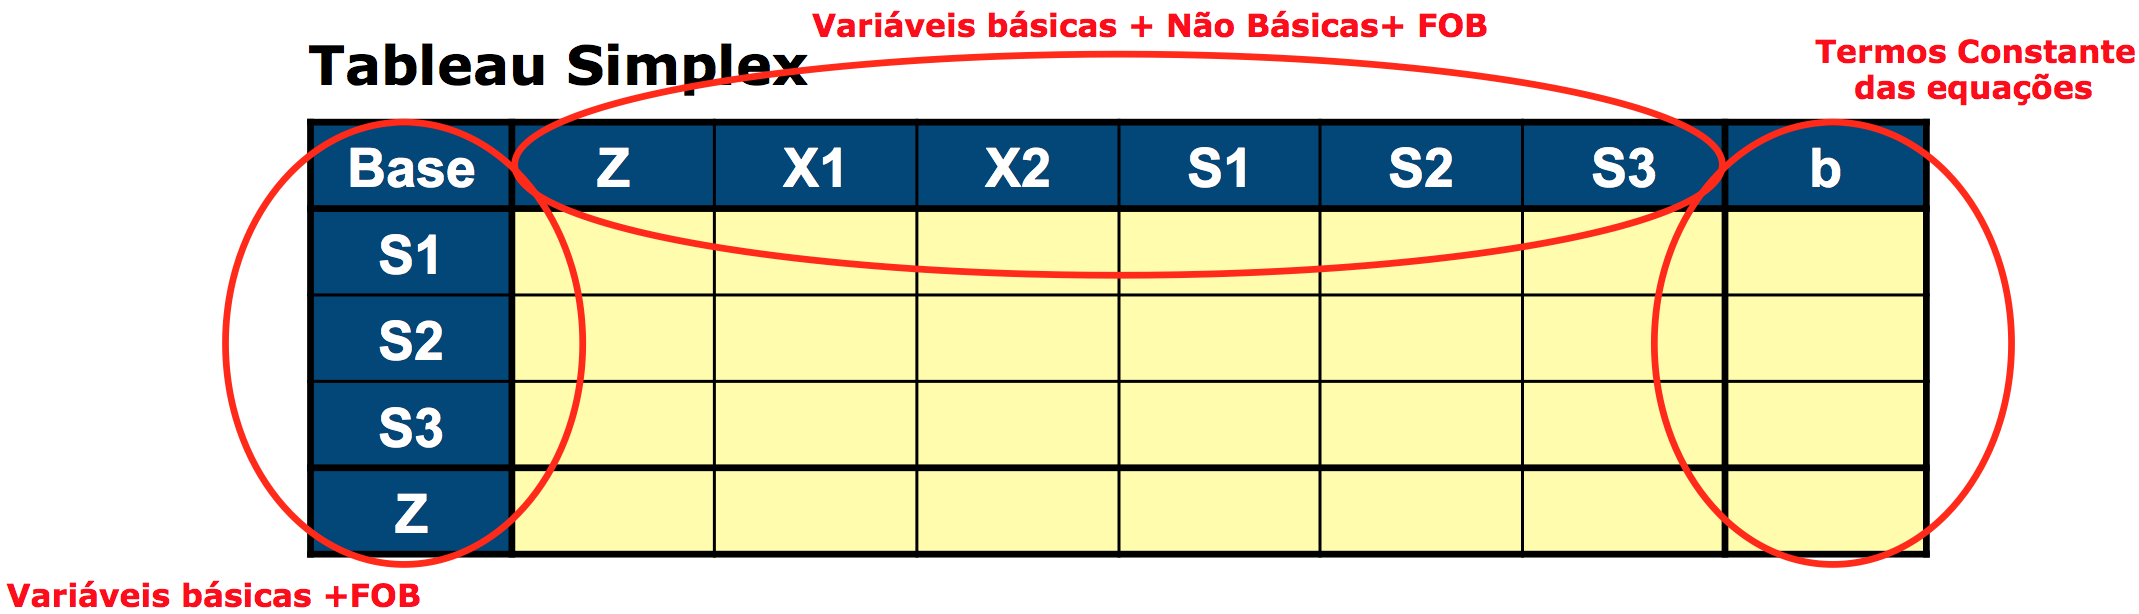
\includegraphics[width=5.2cm,height=2cm]{tableau.png}	
			}		
		\end{column}
	\end{columns}
\end{frame}

\begin{frame}
	\frametitle{
\includegraphics[width=0.6cm,height=0.6cm]{number_4.jpg} \hspace{0.2cm} Passos da Resolução do PPL via Tableau Simplex}
		
	\begin{table}
		\begin{tabular}{c}
			\cellcolor{yellow}Problema em Análise \\
			$
				\begin{matrix}
					\color{red} \max Z - 3x_1 - 5x_2 = 0 \\
					\text{Sujeito a:} \\
					x_1 + {\color{red}S_1 =} 4 \\
					2x_2 + {\color{red}S_2 =} 12 \\
					3x_1 + 2x_2 + {\color{red}S_3 =} 18 \\
					x_1, x_2,{\color{red} S_1, S_2, S_3} \ge 0 \\
				\end{matrix} 	
			$ 
		\end{tabular}
	\end{table}
		
	\begin{table}		
		\caption{\textbf{Tableau Simplex} \color{red} \scriptsize Preenchimento pelas linhas do Tableau	}
		\begin{tabular}{c | c | c | c | c | c | c | c | c | }
			\cline{2-9} 
			&\cellcolor{blue!100} \color{white}Base 
			&\cellcolor{blue!100} \color{white}Z 
			&\cellcolor{blue!100} \color{white} $X_1$ 
			&\cellcolor{blue!100} \color{white} $ X_2$ 
			&\cellcolor{blue!100} \color{white} $S_1$ 
			&\cellcolor{blue!100} \color{white} $S_2$ 
			&\cellcolor{blue!100} \color{white} $S_3$ 
			&\cellcolor{blue!100} \color{white} b \\
			\cline{2-9}
			\color{red} \scriptsize Restr.(1)  
			& \cellcolor{blue!100} \color{white} $S_1$
			& \cellcolor{yellow!50} \only<2->{$0$}
			& \cellcolor{yellow!50} \only<3->{$1$}
			& \cellcolor{yellow!50} \only<4->{$0$}
			& \cellcolor{yellow!50} \only<5->{$1$}
			& \cellcolor{yellow!50} \only<6->{$0$}
			& \cellcolor{yellow!50} \only<7->{$0$}
			& \cellcolor{yellow!50} \only<8->{$4$} \\
			\cline{2-9} 
			\color{red} \scriptsize Restr.(2)  
			& \cellcolor{blue!100} \color{white} $S_2$
			& \cellcolor{yellow!50} \only<9->{$0$}
			& \cellcolor{yellow!50} \only<10->{$0$}
			& \cellcolor{yellow!50} \only<11->{$2$}
			& \cellcolor{yellow!50} \only<12->{$0$}			
			& \cellcolor{yellow!50} \only<13->{$1$}
			& \cellcolor{yellow!50} \only<14->{$0$}
			& \cellcolor{yellow!50} \only<15->{$12$} \\
			\cline{2-9} 
			\color{red} \scriptsize Restr.(3)  
			& \cellcolor{blue!100} \color{white} $S_3$
			& \cellcolor{yellow!50} \only<16->{$0$}
			& \cellcolor{yellow!50} \only<17->{$3$}
			& \cellcolor{yellow!50} \only<18->{$2$}
			& \cellcolor{yellow!50} \only<19->{$0$}
			& \cellcolor{yellow!50} \only<20->{$0$}
			& \cellcolor{yellow!50} \only<21->{$1$}
			& \cellcolor{yellow!50} \only<22->{$18$} \\
			\cline{2-9}
			\color{red} \scriptsize FOB
			\footnote{\color{red}\textbf{A FOB deve ser sempre formada por VNB}}
			& \cellcolor{blue!100} \color{white} $Z$
			& \cellcolor{yellow!50} \only<22->{$1$}
			& \cellcolor{yellow!50} \only<22->{$-3$}
			& \cellcolor{yellow!50} \only<22->{$-5$}
			& \cellcolor{yellow!50} \only<22->{$0$}
			& \cellcolor{yellow!50} \only<22->{$0$}
			& \cellcolor{yellow!50} \only<22->{$0$}
			& \cellcolor{yellow!50} \only<22->{$0$} \\
			\cline{2-9} 
		\end{tabular}
	\end{table}
\end{frame}
